\begin{frame}
	\frametitle{GPIO Keyboard with Note Velocity}
	\centering
	\begin{tikzpicture}
		\path[use as bounding box] (1,-6) rectangle (-8,1);
		\draw [rotate=0] (0,0) -- (0,0.5) -- (-7,0.5) to[out=180,in=90] (-7,0.3) -- (-7,-0.5) -- (-4,-0.5) -- (-4,0) -- cycle;
		\fill (-1,-0.35) rectangle +(0.4,0.2) +(0.1,0) rectangle +(0.3,0.35);
		\draw (-1,-0.25) -- +(-0.1,-0.1);
		\draw (-0.6,-0.25) -- +(0.1,-0.1);
		
		\fill (-6.5,-1.4) rectangle +(0.4,0.2) +(0.1,0) rectangle +(0.3,0.35);
		\draw (-6.5,-1.3) -- +(-0.1,-0.1);
		\draw (-6.1,-1.3) -- +(0.1,-0.1);
		
		\draw (-0.8,-2) -- +(0,-1.5);
		\draw (-6.3,-2) -- +(0,-1.5);
		
	\end{tikzpicture}
\end{frame}
\begin{frame}
	\frametitle{GPIO Keyboard with Note Velocity}
	\centering
	\begin{tikzpicture}
		\path[use as bounding box] (1,-6) rectangle (-8,1);
		\draw [rotate=1] (0,0) -- (0,0.5) -- (-7,0.5) to[out=180,in=90] (-7,0.3) -- (-7,-0.5) -- (-4,-0.5) -- (-4,0) -- cycle;
		\fill (-1,-0.35) rectangle +(0.4,0.2) +(0.1,0) rectangle +(0.3,0.33);
		\draw (-1,-0.25) -- +(-0.1,-0.1);
		\draw (-0.6,-0.25) -- +(0.1,-0.1);
		
		\fill (-6.5,-1.4) rectangle +(0.4,0.2) +(0.1,0) rectangle +(0.3,0.35);
		\draw (-6.5,-1.3) -- +(-0.1,-0.1);
		\draw (-6.1,-1.3) -- +(0.1,-0.1);
		
		\draw (-0.8,-2) -- +(0,-1.5);
		\draw (-6.3,-2) -- +(0,-1.5);
		
		\draw[line width=1em] (-0.8,-2.3) -- +(0,0.3);
		
	\end{tikzpicture}
\end{frame}
\begin{frame}
	\frametitle{GPIO Keyboard with Note Velocity}
	\centering
	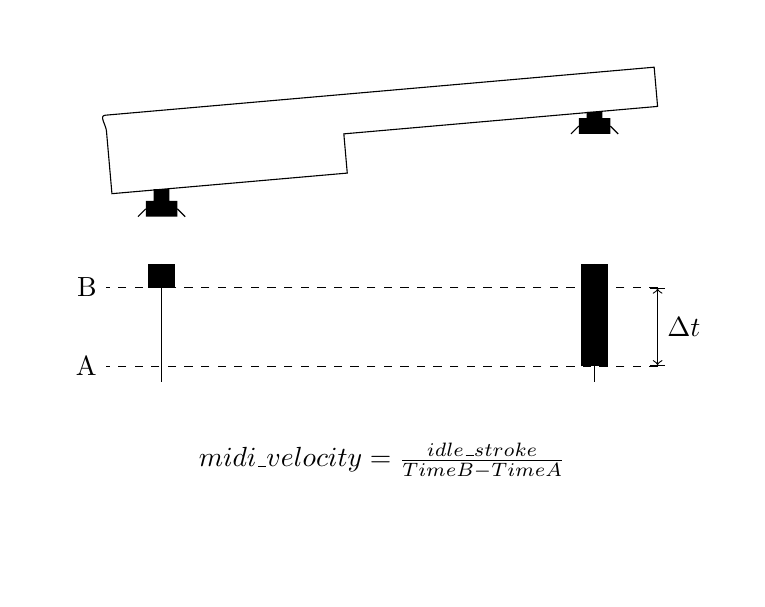
\begin{tikzpicture}
		\path[use as bounding box] (1,-6) rectangle (-8,1);
		\draw [rotate=5] (0,0) -- (0,0.5) -- (-7,0.5) to[out=180,in=90] (-7,0.3) -- (-7,-0.5) -- (-4,-0.5) -- (-4,0) -- cycle;
		\fill (-1,-0.35) rectangle +(0.4,0.2) +(0.1,0) rectangle +(0.3,0.28);
		\draw (-1,-0.25) -- +(-0.1,-0.1);
		\draw (-0.6,-0.25) -- +(0.1,-0.1);
		
		\fill (-6.5,-1.4) rectangle +(0.4,0.2) +(0.1,0) rectangle +(0.3,0.35);
		\draw (-6.5,-1.3) -- +(-0.1,-0.1);
		\draw (-6.1,-1.3) -- +(0.1,-0.1);
		
		\draw (-0.8,-2) -- +(0,-1.5);
		\draw (-6.3,-2) -- +(0,-1.5);
		\draw[line width=1em] (-6.3,-2.3) -- +(0,0.3);
		\draw[line width=1em] (-0.8,-3.3) -- +(0,1.3);
		
		\pause
		
		\draw[dashed] (0,-2.3) -- +(-7,0);
		\draw[dashed] (0,-3.3) -- +(-7,0);
		
		
		\draw[|<->|] (0,-2.3) -- node[right]{$\Delta t$} +(0,-1);
		
		\node[left] at (-7,-2.3){B};
		\node[left] at (-7,-3.3){A};
		
		\node at (-3.5,-4.5) {$\text{midi\_velocity}=\frac{\text{idle\_stroke}}{\text{Time B - Time A}}$};
	\end{tikzpicture}
\end{frame}

\begin{frame}{state machine}
	\centering
	\begin{tikzpicture}[node distance=4cm,bend angle=10]
        \node[state,minimum size=1.8cm]   (act) {active};
        \node[state,minimum size=1.8cm]   (touch) [below right of=act] {touched};
        \node[state,minimum size=1.8cm]   (press) [below left of=act] {pressed};
		
		\path[-latex] (act) edge[bend left] node[sloped,above] {$b_1|$start} (touch)
						(touch) edge node[sloped,below] {$b_2|$send} (press)
								edge[bend left] node[sloped,below] {$\neg b_1|$off} (act)
						(press) edge node[sloped,above] {$\neg b_1|$off} (act);
		\path[-latex] (press) edge [loop below] node {$b_2|$on\&off} ();
		\path[-latex] (act) edge [loop left] node {$\neg b_1|$off} ();
	\end{tikzpicture}
\end{frame}

\begin{frame}
  \frametitle{CMIDID Kernel Module}
  \centering
  \begin{tikzpicture}
    \node at (0, 0) {
\includegraphics[width=4cm]{img/tux-on-eighth-note.jpg}};
    \node[rotate=90] at (-5, 0) {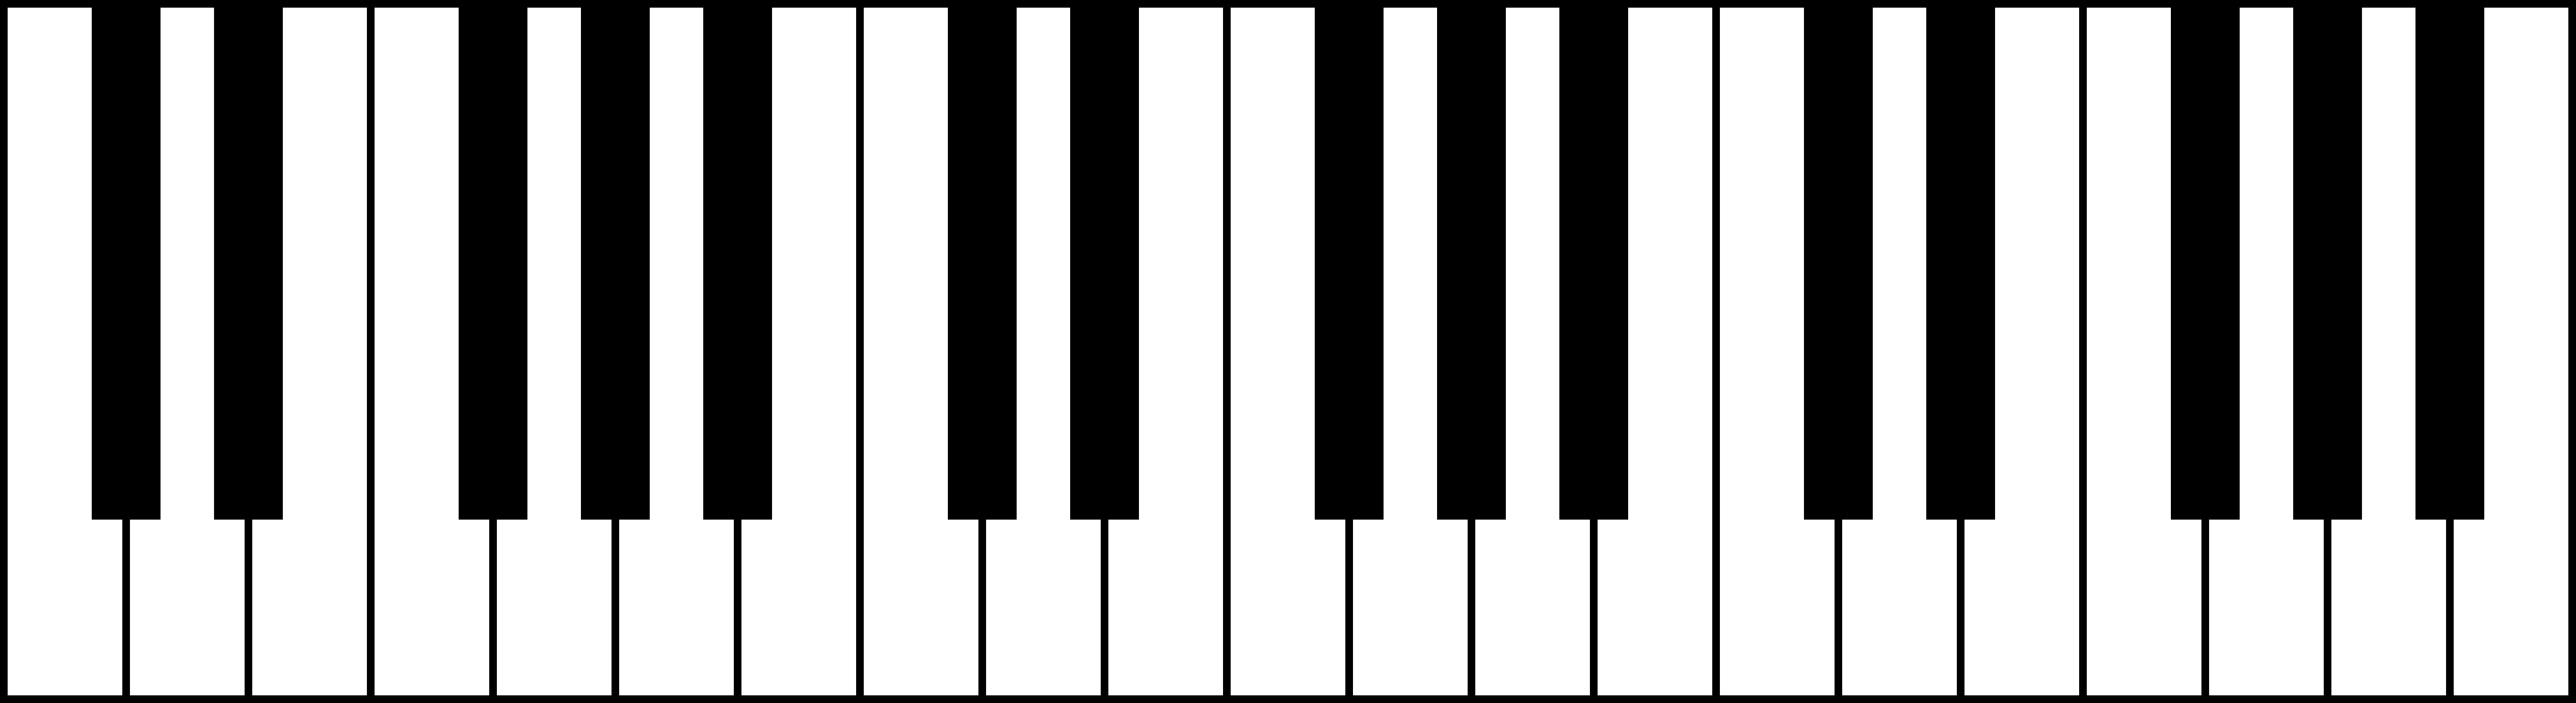
\includegraphics[width=4cm]{img/Musical_keyboard.png}};
    \node[align=center, text width=4cm] at (-3, 2.4) {GPIO Interrupts};
    \draw[ultra thick, ->] (-4, 1.5) -- (-2, 1.5);
    \draw[ultra thick, ->] (-4, .75) -- (-2, .75);
    \draw[ultra thick, ->] (-4, 0) -- (-2, 0);
    \draw[ultra thick, ->] (-4, -.75) -- (-2, -.75);
    \draw[ultra thick, ->] (-4, -1.5) -- (-2, -1.5);
    \node[align=center, text width=4cm] at (0,-2.2) {CMIDID Module};
    \draw[ultra thick, ->] (2, 0) -- (2.5, 0);
    \node[text width=2cm, draw] at (4, 0) {ALSA\\Sequencer\\Interface};
    \node[text width=4cm, align=center, rotate=270] at (2.2, -0.2) {MIDI\qquad Events};
  \end{tikzpicture}
\end{frame}

\begin{frame}{features}
	module parameters
	\begin{itemize}
		\item mapping of GPIO pins to notes
		\item button debounce timeout
	\end{itemize}
	\pause
	\texttt{ioctl} features
	\begin{itemize}
		\item calibrate velocity
		\begin{itemize}
			\item minimal
			\item maximal
		\end{itemize}
		\item transpose
		\item velocity curves
	\end{itemize}
\end{frame}

\begin{frame}{velocity curves}
	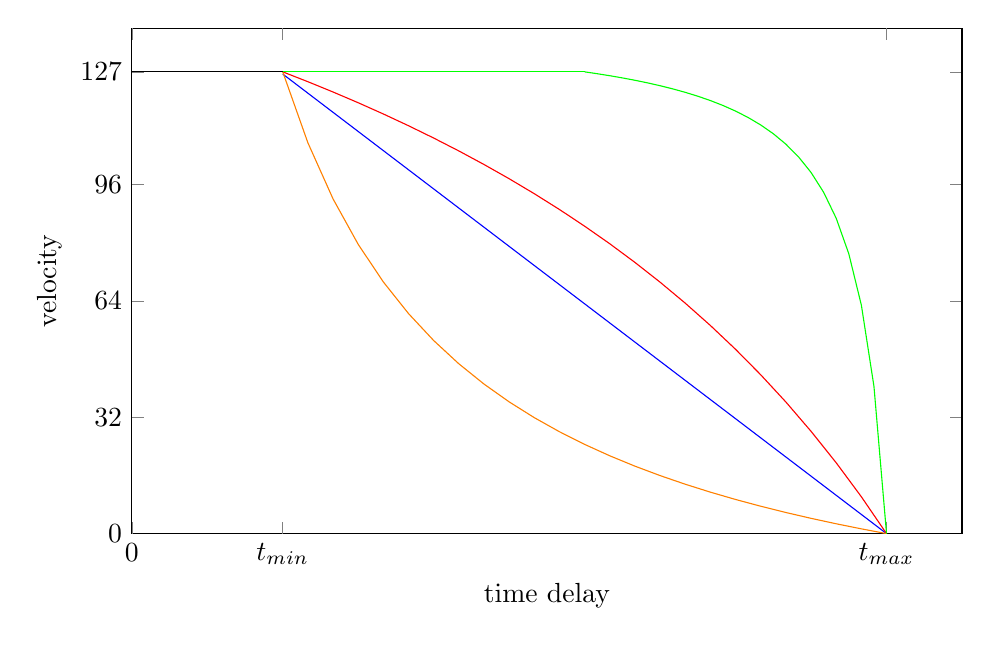
\begin{tikzpicture}
		\begin{axis}[width=\textwidth,xtick=\empty,extra x ticks={0,20,100},extra x tick labels={$0$,$t_{min}$,$t_{max}$},ytick={0,32,64,96,127},height=8cm,ymin=0,ymax=139,xmin=0,xmax=110,ylabel={velocity},xlabel={time delay},log basis y={2}]
			\addplot[draw=blue,domain=20:100] {-1.58*x+158};
			\addplot[draw=red,domain=20:100] {20560.6/(x - 180.63) + 255};
			\addplot[draw=orange,domain=20:100] {4207.87/(x + 5.19685) - 40};
			\addplot[draw=green,domain=60:100] {573.228/(x - 104.094) + 140};
			\addplot[draw=black,domain=0:20] {127};
			\addplot[draw=green,domain=20:60] {127};
		\end{axis}
	\end{tikzpicture}
\end{frame}
		
		%\draw [rotate=5] (0,0.5) -- (0.1,0.7) -- (-5,0.7) -- +(0.05,0.1) -- (-6.85,0.8) to[out=180,in=90] (-6.85,0.6);
		%\node at (-4,2) {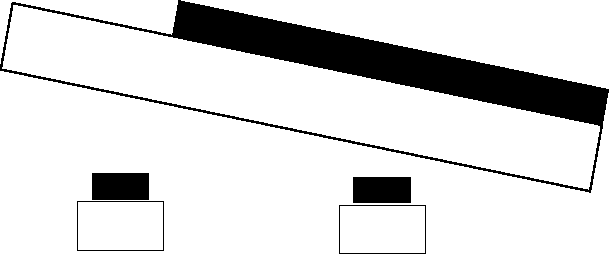
\includegraphics[width=4cm]{img/key1.pdf}};
		%\node[align=left ,text width=4cm] at (1,2) { Two buttons connected \\ to GPIO ports};
		%\node at (-4,0) {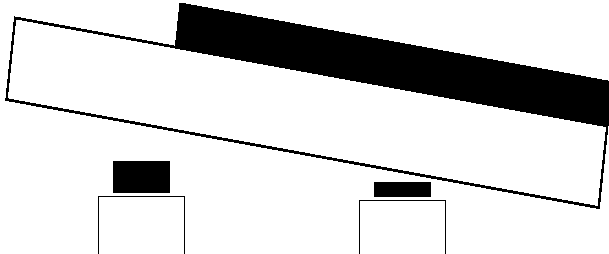
\includegraphics[width=4cm ]{img/key2.pdf}};
		%\node[align=left ,text width=4cm] at (1,0) { Interrupt Time A};
		%\node at (-4,-2) {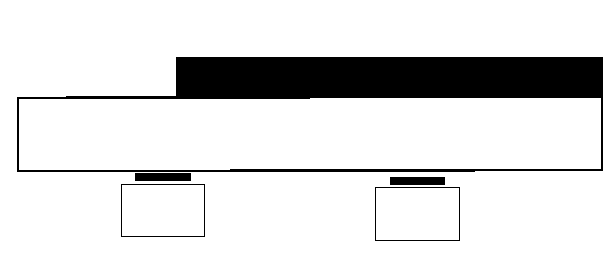
\includegraphics[width=4cm]{img/key3.pdf}};
		%\node[align=left ,text width=4cm] at (1,-2) { Interrupt Time B};
		%\node[align=left ,text width=6cm] at (-1,-3.5) {  $midi\_velocity=\frac{idle\_stroke}{Time B - Time A}$};


%\begin{frame}
%	\frametitle{ALSA}
%	\centering
%  	\begin{tikzpicture}
%		\node at(0,0) {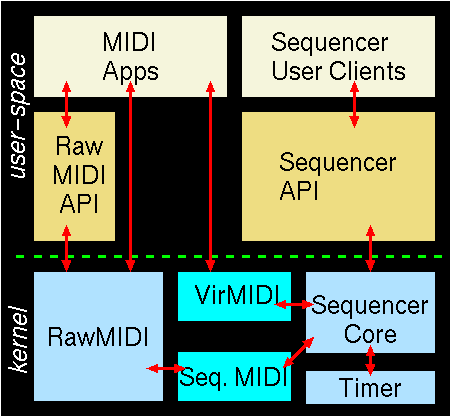
\includegraphics[width=6cm]{img/alsa.png}};
%		\pause
%		\fill[opacity=0.7,fill=white] (-4,-4) -- (-4,4) -- (4,4) -- (4,-0.7) -- (0.95,-0.7) -- (0.95,-2.08) -- (2.92,-2.08) -- (2.92,-0.7) -- (4,-0.7) -- (4,-4) -- cycle;
%		%\draw[ultra thick, color= pink] (2.9, -2.1) rectangle (0.9,-0.7);
%	\end{tikzpicture}
%\end{frame}

%\begin{frame}[fragile]
%	\frametitle{ALSA sequencer connection manager}
%Input devices (\texttt{aconnect -i}):
%  	\begin{lstlisting}
%client 20: 'cmidid-client' [type=kernel] 
%    0 'cmididpinfo    
%	\end{lstlisting}
%Output devices (\texttt{aconnect -o}):
%  	\begin{lstlisting}
%client 128: 'FLUID Synth (2274)' [type=user]
%    0 'Synth input port (2274:0)'
%\end{lstlisting}
%$ $
%\\
%Connect both ports with \texttt{aconnect 20:0 128:00}
%
%
%
%\end{frame}

%\begin{frame}
%	\frametitle{Why Kernel Module?}
%\begin{tikzpicture}
%	\path[use as bounding box] (-8,2) rectangle (-3,-6);
%	\node at (-6.7cm,0) {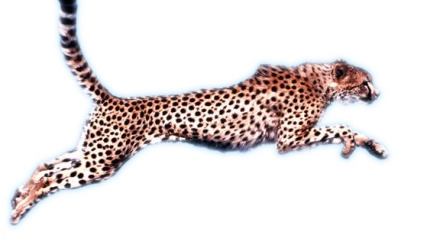
\includegraphics[width=8cm]{img/cheetah.png}};
%	\node[text width=7cm] at(-2,-3) {
%	\begin{itemize} 
%		\item precise timers (1 ns resolution) 
%		\item usage of interrupts $\Rightarrow$ short delay
%		\item relativley small overhead 
%	\end{itemize}};
%\end{tikzpicture}
%\end{frame} 
%